\chapter{System Design Overview}\label{c:sys-design}

\section{Cryostat Design}\label{s-cryo-design}

The cryostat for the \Imager\ was designed with the goals of simplicity, reliability and turn-key automated operation.
Highly reliable and easy-to-use cryogen-free mechanical cryocoolers are commercially available, but these cryocoolers are seldom capable of reaching temperatures below 2.5~K.
Reaching sub-Kelvin temperatures requires a second refrigeration stage, which in our case is a He-4 adsorption refrigerator.
The He-4 adsorption refrigerator is based on a proven design and its use can easily be automated.
Three temperature stages within the cryostat are provided in order to provide intercepts for heat sinking wiring and other objects that are thermal connected to room temperature. 
The result is a reliable cryogen-free cryogenic system that can be controlled remotely.

xxx next para needs rewriting - need to explain what PTC is early on. maybe next para needs to move here, somewhat rewritten.

The cryostat itself was built by Precision Cryogenics\footnote{Precision Cryogenics Systems, Inc. Indianapolis, IN. \url{http://www.precisioncryo.com}} to designs provided by the \Imager\ team.
\figref{fig:cryo-cutaway} shows a cutaway view of the cryostat, and \tableref{tab:temp-optical-load} lists the temperatures typically reached by different parts of the cryostat during operation when the cryostat is open optically.
The cryostat has two main parts: a cylinder containing both the PTC and the \He4-adsorption refrigerator, and a box located at the bottom of the cylinder which contains temperature intercept plates and the focal plane.
There are three temperature stages, the ``90~K'' Cold Plate, the ``4~K'' Cold Plate, and the Focal Plane.
The PTC 1st stage is connected to the ``90~K'' Cold Plate by a tube of Al 1100 and a set of CDA-101 Cu braids.
The combination of this long thermal path with the high heat load on the optical filters sunk to the ``90~K'' stage explains the 45~K temperature differential between the ``90~K`` cold plate and the PTC 1st stage.
The PTC 2nd stage is connected to the ``4 K'' Cold Plate by a large (3.0 in diameter by 2.78 in long) cylinder of CDA-110 Cu\footnote{This cryostat was originally designed to work with a different cryocooler. The PTC currently installed had a shorter distance between the 1st and 2nd stages, necessitating the Cu cylinder to take up this extra space}, followed by tube of alloy CDA-101 Cu followed by a set of  CDA-101 copper braids.
The Cu tube is broken into two halves, and the condensation plate (see below) of the adsorption fridge is clamped between these two halves. The ``90 K'' Cold Plate is stood off from the cryostat vacuum jacket by four ``roll wrapped'' carbon fiber tube standoffs. The ``4~K'' Cold Plate stands off from the ``90 K'' Cold Plate by eight supports made of G-10.

The first two temperature intercept stages are provided by a Cryomech PT407 Pulse Tube Cryorefrigerator\footnote{Cryomech, Inc. Syracuse, NY. \url{http://www.cryomech.com}}
The PT407 has two cooling stages.
The first stage has 25~W of cooling power at 55~K while the second stage has 0.7~W at 4.2 K.
Our PT407 uses a remote motor, so that the cold head attached to the cryostat has no moving parts, minimizing vibration of the cryostat.
Vibration of the cryostat can lead to microphonic pickup either directly in the detectors themselves or in the readout circuitry, leading to much higher detector noise.

\begin{figure*}
\centering
\begin{tikzpicture}
    \node[anchor=south west,inner sep=0] (image) at (0,0) {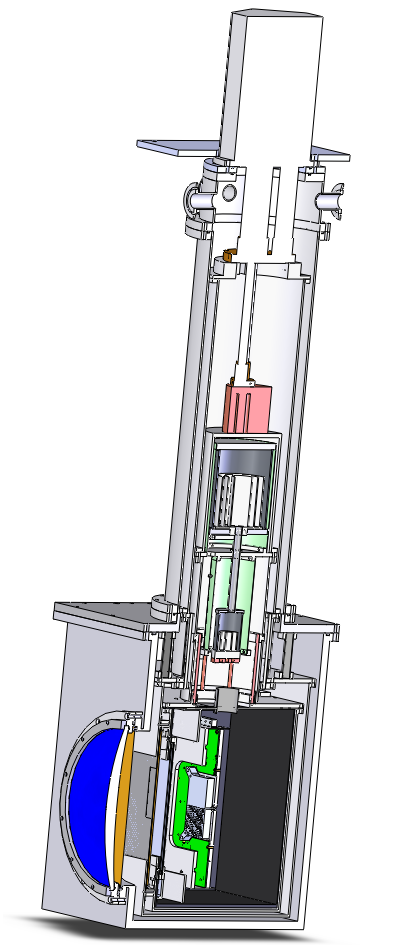
\includegraphics[width=2.6in]{./images/cryostat-cutaway.png}};
    \begin{scope}[x={(image.south east)},y={(image.north west)}]
	    %\draw[help lines,xstep=.1,ystep=.1] (0,0) grid (1.5,1);
		%\foreach \x in {0,1,...,15} { \node [anchor=north] at (\x/10,0) {0.\x}; }
		%\foreach \y in {0,1,...,9} { \node [anchor=east] at (0,\y/10) {0.\y}; }
		
        \draw[red,ultra thick,rounded corners] (0.50,0.7) rectangle (0.85,0.75) node[below left] {\textbf{A}}; % PTC407 1st stage CH
        \draw[red,ultra thick,rounded corners] (0.56,0.595) rectangle (0.71,0.64) node[below left] {\textbf{B}}; % PTC407 2st stage CH
        \draw[red,ultra thick,rounded corners] (0.53,0.55) rectangle (0.78,0.595) node[below left] {\textbf{C}}; % Cu Cylinder
        \draw[red,ultra thick,rounded corners] (0.505,0.32) rectangle (0.75,0.55) node at +(-0.1,-0.03) {\textbf{D}}; % sorp fridge
        \draw[red,ultra thick,rounded corners] (0.4,0.06) rectangle (0.70,0.26) node[red,below left] {\textbf{E}}; % Focal Plane
        
        \draw[thick,<->] (1.05,0.04) -- +(0,0.31) node[midway,right] {18 in}; % scale bar
    \end{scope}
\end{tikzpicture}
\caption{Cutaway view of the \Imager. \textbf{A} PT407 1st stage cold head \textbf{B} PT407 2nd stage cold head \textbf{c} Cu cylinder connected PT407 2\textsuperscript{nd} stage cold head to Cu tube, which then connects to \He4-sorption refrigerator condensation plate. \textbf{D} \He4-sorption refrigerator \textbf{E} Focal Plane. Copper ropes connecting focal plane to 1~K cold plate are not visible in this view.}
\label{fig:cryo-cutaway}
\end{figure*}

\begin{table*}
\centering
\caption{Temperatures Reached Under Optical Load xxx should I add temps when closed optically?}
\label{tab:temp-optical-load}
\begin{tabular}{l r}
\toprule
Temperature Stage &  Temperature (K)\\
\midrule
PTC 1st Stage Cold Head 			& 48 \\
PTC 2st Stage Cold Head 			& 3.5 \\
Cryostat ``50 K'' Cold Plate 		& 84 \\
Cryostat ``4 K'' Cold Plate 			& 5.8 \\
Adsorption Fridge Condensation Plate 	& 3.7 \\
Focal Plane 						& 0.962 \\
\bottomrule
\end{tabular}
\end{table*}

Options for reaching temperatures below the $\sim$1.2~K transition temperature of our \TES\ detectors include: dilution refrigerators, adiabatic magnetization refrigerators, pumped \He4 baths, and \He3- and/or \He4-adsorption refrigerators.
We chose a \He4-adsorption fridge because of its low cost, ease of operation compared to other solutions, and the fact that the typical base temperatures under no load of \abt{\SI{700}{\mK}} is well-matched to our application. xxx actually the key point is temperature - others are in addition.
A  \He4-sorption fridge works by using a charcoal adsorber to pump on a bath of liquid \He4, reducing the \He4 boiling point and thus the temperature of the bath.
The \He4 is contained withing a sealed reservoir so that the refrigerator acts as a closed system requiring no \He4 replenishment. 
While \He4-sorption fridges are commercially available, our team choose to design and build a custom fridge based on a design that has been proven in astronomical applications\cite{devlin_high_2004}.

\figref{fig:he4sorp} shows a schematic depiction of the \Imager's \He4-sorption refrigerator.
The entire refrigerator is filled with 2.07~moles of \He4 gas, giving a pressure of 900~psi at room temperature.
In normal operation the heat switch between the charcoal pumping chamber (``pump'') and the \He4 condensation plate is closed, keeping the charcoal as cold as possible in order to adsorb as much \He4 as possible, keeping the temperature of the cold plate as low as possible.

\begin{figure*}
\centering
\begin{tikzpicture}
    \node[anchor=south west,inner sep=0] (image) at (0,0) {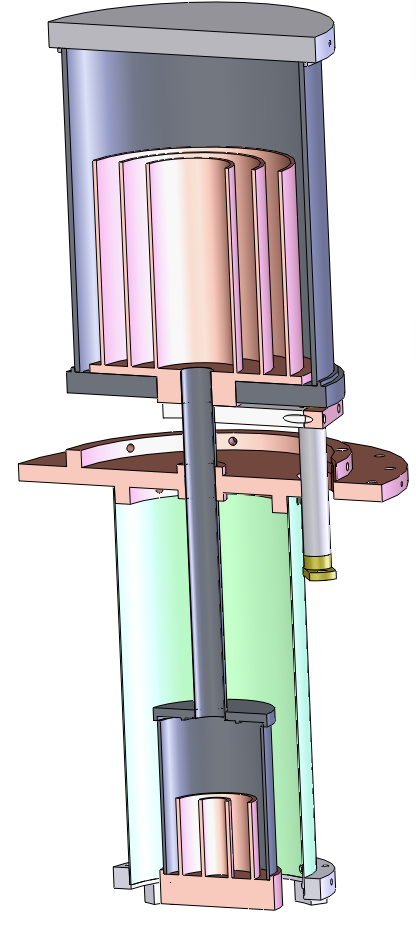
\includegraphics[width=3.0in]{./images/he4-sorp-fridge-cutaway.png}};
    \begin{scope}[x={(image.south east)},y={(image.north west)}]
	    %\draw[help lines,xstep=.1,ystep=.1] (0,0) grid (1.5,1);
		%\foreach \x in {0,1,...,15} { \node [anchor=north] at (\x/10,0) {0.\x}; }
		%\foreach \y in {0,1,...,9} { \node [anchor=east] at (0,\y/10) {0.\y}; }
        \draw[blue,ultra thick,rounded corners] (0.10,0.56) rectangle (0.86,1.01) node[below left] {\textbf{A}}; % pump
        \draw[blue,ultra thick,rounded corners] (0.02,0.56) rectangle (1.03,0.44) node[above left] {\textbf{B}}; % cond plate
        \draw[blue,ultra thick,rounded corners] (0.70,0.56) rectangle (0.88,0.36) node[above left] {\textbf{C}}; % heat switch
        \draw[blue,ultra thick,rounded corners] (0.35,0.25) rectangle (0.72,-0.02) node[above left] {\textbf{D}}; % pot
        
		\draw[thick,<->] (0.9,0.02) -- ++(0,0.21875) node[midway,right] {3 in}; % scale bar
    \end{scope}
\end{tikzpicture}
\caption{Cutaway view of the \He4-sorption refrigerator. \textbf{A} Charcoal pumping chamber (``pump''). The charcoal is attached to the concentric copper cylinders. Cylinders are used to maximize the surface area covered by the charcoal. \textbf{B} Condensation plate. This copper plate is kept below the boiling point of \He4 in order to provide a point in the refrigerator for \He4 to condense and drip into the condensation pot. \textbf{C} \He4 gas gap heat switch. This heat switch is used to cool the charcoal in order to pump on the \He4 bath in the condensation pot. \textbf{B} \He4 condensation pot (``pot''). The condensed \He4 accumulates here. The concentric cylinders provide additional surface area for thermal contact to the liquid \He4. Not shown is a small (xxx check size from Bob) constriction in the stainless steel tube connecting the pump and pot, intended to restrict the flow of superfluid \He4 away from the pot.}
\label{fig:he4sorp}
\end{figure*}

Cycling the refrigerator requires four steps.
First the heat switch is opened.
The \He4-sorption refrigerator uses a \He4 gas-gap heat switch manufactured by Chase Cryogenics\footnote{Chase Research Cryogenics, Ltd. Sheffield, UK}, which requires 5 minutes of waiting time in order for the switch to fully open.
Second, the pump is heated by applying \SI{5}{\W} via a \SI{500}{\ohm} power resistor.
This power is applied until the temperature of the pump reaches 40 K, which is high enough to drive nearly all of the adsorbed \He4 off of the charcoal.
Third, the power to the pump is turned off.
Once the temperature of the condensation plate falls below the boiling point of \He4, \He4 will begin to condense on its walls, dripping into the \He4 condensation pot (``pot'').
Fourth, once the temperature of the pot has fallen to 4.0~K, the heat switch is turned back on.
This cools the pump, allowing \He4 to again adsorb onto the charcoal, which has the effect of pumping strongly on the pot, and cooling the \He4 contained there to the base temperature of $\sim$ 970~mK under optical load.
This process is easy to automate, and a LabView program cycles the fridge automatically every night while the system is operating.

Under optical load, a full cycle of the \He4-sorption refrigerator takes approximately 4 hours, reaching a base temperature of $\sim$~970~mK.
When no additional load is applied the hold time is 9 hours.
When the temperature of the stage is held at the typical operating temperature of 1100~mK the hold time is only 3:45 hours.

\tableref{tab:fp-thermal-load} shows the predicted heat load on the \He4-sorption refrigerator.
It excludes parasitic load inherent to the sorption refrigerator itself. xxx mention parasitic load here?

xxx - include data on temp vs load for the fridge?

\begin{table*}[ht]
\centering
\caption{Predicted Thermal Load on 1~K Stage. These calculations assume that the readout wiring and Ti-6Al-4V spiders are running from 6.4~K to 1.0~K.}
\label{tab:fp-thermal-load}
\begin{tabular}{@{}lrr@{}}
\toprule
 & \multicolumn{2}{c}{Predicted Thermal Load} \\
\cmidrule(r){2-3}
Heat Load Source & 1004 Detectors (\si{\uW}) &  251 Detectors (\si{\uW}) \\
\midrule
Readout wiring 								& 50 & 125 \\
Series array \SQUID\ modules 		& xxx & xxx \\
\SQUID\ multiplexing chips 				& xxx & xxx \\
Detectors shunt resistors 			& 5 & 18 \\
Detectors (Optical + Electrical)		& 0.25 & 1 \\
Ti-6Al-4V spiders 							& 130 & 130 \\
Out-of-band optical power 			& xxx & xxx \\
\midrule
Total												& 185 + xxx & 274 + xxx \\
\bottomrule
\end{tabular}
\end{table*}

% xxx - I get 500 uW for the load from the four BOSE wires (300 K -
% 1K). Need to add them to the table. Can this be correct? I'm sure I did this calculation in the past and got a much smaller number. Did I screw up in the past? Is today's calculation in error? Am I intercepting this load at 50~K or 4~K, and I forgot about that? Did I use a much longer wire than 1~m? This could be a big cryogenic problem!

\section{Optical Design}\label{sec:ch4-optical-design}

Because I did not design the optical system, this section merely summarizes information about the optical system required for understanding the remainder of this thesis.

The optical system is a Cassegrain design.
A Cassegrain design was chosen because circular symmetry makes these systems easy to design for on-axis performace at finite distances%
\footnote{William Duncan, personal communication}.
\figref{fig:ch4-optical-schematic} shows a schematic of the optical system including the focal plane.
Light enters the system from the left in this schematic, and bounces off the primary mirror onto the secondary mirror.
From the secondary mirror the light passes through a hole in the center of the primary mirror and through a window into the cryostat.
The cryostat window is a high-density polyethylene (\HDPE) lens that makes the system telecentric; this means that focal surface of the system inside the cryostat is planar, not curved, and simplifies the design of the detector focal plane.
On the focal plane itself, light is captured by smooth-walled conical feedhorns (see \sectionref{sec:ch4-feedhorn-design}) which funnel the light onto the detectors.

\begin{figure*}
\centering
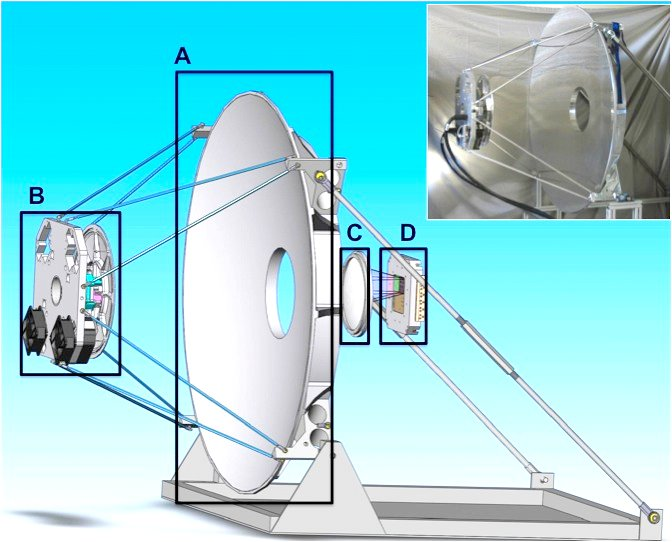
\includegraphics[width=4in]{images/optics-labeled-fixed.jpg}
\caption{
Schematic showing elements of optical system.
\textbf{A} \SI{1.3}{\m} elliptical primary mirror.
\textbf{B} Platform on which secondary mirror is mounted.
\textbf{C} High-density-polyethylene (\HDPE) window leading into cryostat.
           This window acts as a lens to make the system telecentric.
\textbf{D} Detector focal plane package.
           The lid covering the focal plane holds an optical filter which defines the band of observation; see \sectionref{xxx}.
}
\label{fig:ch4-optical-schematic}
\end{figure*}

\tableref{tab:ch4-optical-specs} lists imporant properties and parameters for the optical elements of the system.
The most important paramter is the \SI{1.3}{\m} diameter of the primary mirror; this sets the resolution of the overall system.
\figref{fig:ch4-spot-diagrams} shows spot diagrams for the optical system generated by a \ZEMAX\ model for the system focused at \SI{16}{\m}.
They demonstrate the the system's optical performance is diffraction-limited over the entire focal plane for mirror rotations in both directions of up to \ang{1}, the maximum angle the mirror is ever displaced.
\tableref{tab:ch4-zemax-parms} lists important optical properties of the system obtained from the \ZEMAX\ model.

\begin{sidewaystable}[ht]
\centering
\caption{
  Optical system specifications.
  Some of the dimenions and parameters are listed to precisions higher than achievable manufacturing tolerances.
  These dimensions and parameters were chosed by optimization rourtines in \ZEMAX\, and are kept to full precision here for archival purposes.
  The shape of the elliptical and hyperbolic mirrors follows the equation $z(r) = c r^2 / (1 + \sqrt{1 - (1+k) c^2 r^2})$, where $c$ is the inverse of the mirror radius, $k$ is the conic parameter, and $r$ is the radial distance from the center mirrors.
  The lens surfaces follow the equation given in the table.
}
\label{tab:ch4-optical-specs}
\begin{tabular}{p{1.5in} p{1.5in} p{0.7in} p{4.9in} }
\toprule
Optical Element & Type & Outer \newline Diameter & Details \\
\midrule

Primary Mirror    & Elliptical Mirror    & \SI{1.3}{\m} 
    &  Vertex \SI{16}{\m} from farfield focalplane \\
& & &  \ZEMAX\ radius $c^{-1} = \SI{1801.453127}{\mm}$ \\
& & &  \ZEMAX\ conic $k = \num{-0.878728}$ \\
& & &  Semi-major axis: \SI{14.85}{\m} \\
& & &  Semi-minor axis: \SI{5.17}{\m} \\
& & &  Distances from mirror vertex to foci: \SI{0.93}{\m} and \SI{28.8}{\m} \\

Secondary Mirror  & Hyperbolic Mirror    & \SI{0.44}{\m}
    &  Veretex \SI{626.82}{\mm} from primary mirror vertex \\
& & &  \ZEMAX\ radius $c^{-1} = \SI{937.37187}{\mm}$ \\
& & &  \ZEMAX\ conic $k = \num{-4.466172}$ \\
& & &  Eccentricity \num{2.11} \\

Cryostat Window   & \HDPE\ Aspheric Lens & \SI{0.24}{\m}
    &  Outer vertex location depends on focus distance; see \tableref{tab:ch4-zemax-parms} \\
& & &  \SI{2}{\cm} thick at center \\
& & &  Index of refraction $n = \num{1.525}$ \\
& & &  Outer Surface: $z(k) = c r^2 / (1 + \sqrt{1 - c^2 r^2}) + \sum_{k=1}^{k=8} \beta_k r^k$, where 
       $c^{-1} = \SI{-1052.933}{\mm}$,
       $\beta_1 = -\SI{4724.966}{\mm}$,
       $\beta_2 =  (\SI{0}{\mm})^{-2}$,
       $\beta_3 =  (\SI{88.649}{\mm})^{-3}$,
       $\beta_4 = -(\SI{67.854}{\mm})^{-4}$,
       $\beta_5 =  (\SI{90.995}{\mm})^{-5}$,
       $\beta_6 =  (\SI{89.966}{\mm})^{-6}$,
       $\beta_7 = -(\SI{97.618}{\mm})^{-7}$,
       $\beta_8 = -(\SI{191.31}{\mm})^{-8}$ \\
& & &  Inner Surface: $z(k) = c r^2 / (1 + \sqrt{1 - c^2 r^2}) + \sum_{k=1}^{k=8} \beta_k r^k$, where 
       $c^{-1} = \SI{-699.782}{\mm}$,
       $\beta_1 = -\SI{62.359}{\mm}$,
       $\beta_2 =  (\SI{0}{\mm})^{-2}$,
       $\beta_3 = -(\SI{45.520}{\mm})^{-3}$,
       $\beta_4 =  (\SI{59.477}{\mm})^{-4}$,
       $\beta_5 = -(\SI{74.141}{\mm})^{-5}$,
       $\beta_6 =  (\SI{86.306}{\mm})^{-6}$,
       $\beta_7 = -(\SI{107.763}{\mm})^{-7}$,
       $\beta_8 = -(\SI{124.984}{\mm})^{-8}$ \\
Detector Focal Plane &                   & N/A           &  \SI{171.541}{\mm} from vertex of back of cryostat window \\
\bottomrule
\end{tabular}
\end{sidewaystable}

\begin{table*}[ht]
\centering
\caption{
  Parameters of the optical system extracted \ZEMAX\ simulations.
  ``Focus Distance'' is the distance from the apex of the primary mirror at which the system is focused.
  ``Lens Distance'' is the distance from the outer vertex of the len to the vertex of primary.
  ``Plate Scale'' gives the ratio of distances on the far-field focal plane to the detector focal plane.
  ``Mirror Rotation'' give the distance that the on-axis point moves when the mirror is roated by \ang{1}.
  ``F-Number'' Gives the ratio of the focal distance to the aperture size as viewed from the detector focal plane; this the ``Working F/\#'' from \ZEMAX.
  ``Marginal Rays'' give the angle away from the optical axis of the inner/outer marginal rays; these are the most extreme rays emerging from the detector focal plane that reach the far-field focal plane.
}
\label{tab:ch4-zemax-parms}
\begin{tabular}{cccccc}
\toprule
  \specialcell{Focus Distance \\ (\si{\m})} &
  \specialcell{Lens Distance \\ (\si{\mm})} &
  \specialcell{Plate Scale \\ (\si{\cm}/\si{\mm})} &
  \specialcell{Mirror Rotation \\ (\si{\cm}/\si{\degree})} &
  F-Number & 
  \specialcell{Marginal Rays \\ (\si{\degree})} \\
\midrule
16 & 230.475 &  6.111 & 18.354 & 2.01 &  \ang{4.24}  \ang{11.22} \\
17 & 197.18  &  6.638 & 19.330 & 1.96 &  \\ % xxx need marginal rays
28 &   8.0   & 12.589 & 30.037 & 1.71 &  \\ % xxx need marginal rays
\bottomrule
\end{tabular}
\end{table*}

% xxx diagram like fig 4in schwan2011 would be good

\begin{figure*}
\centering
\begin{tabular}{lr}
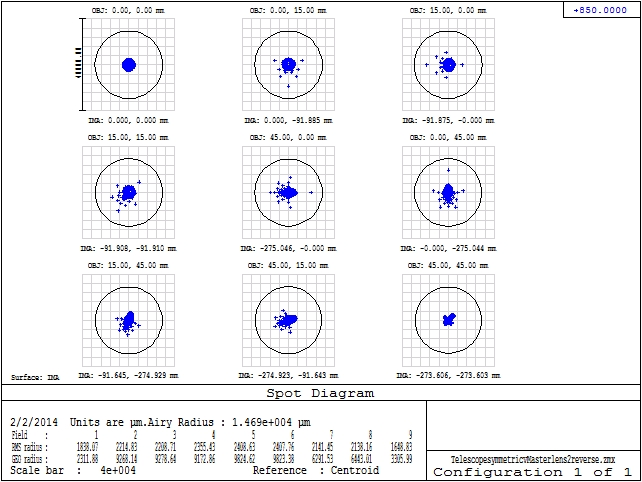
\includegraphics[width=3in]{images/ch4-zemax-spot-0-0.JPG}
 &
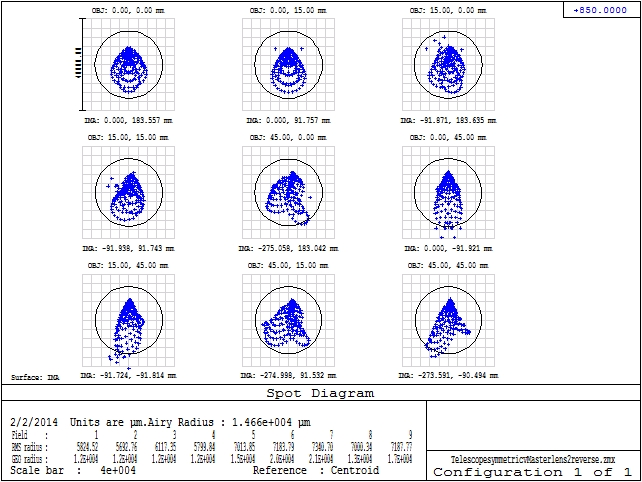
\includegraphics[width=3in]{images/ch4-zemax-spot-1-0.JPG}
 \\
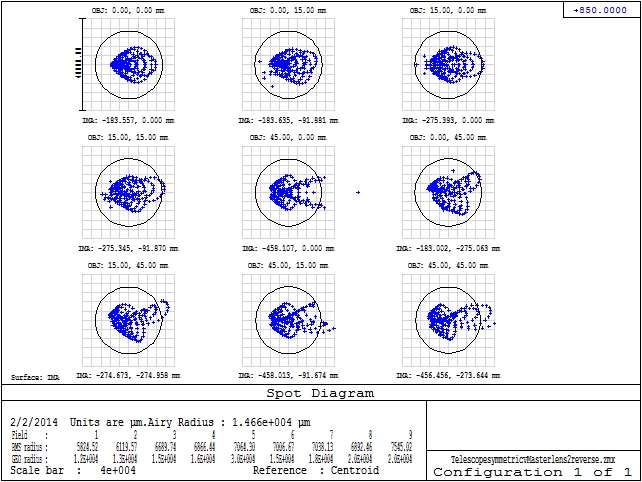
\includegraphics[width=3in]{images/ch4-zemax-spot-0-1.JPG}
 &
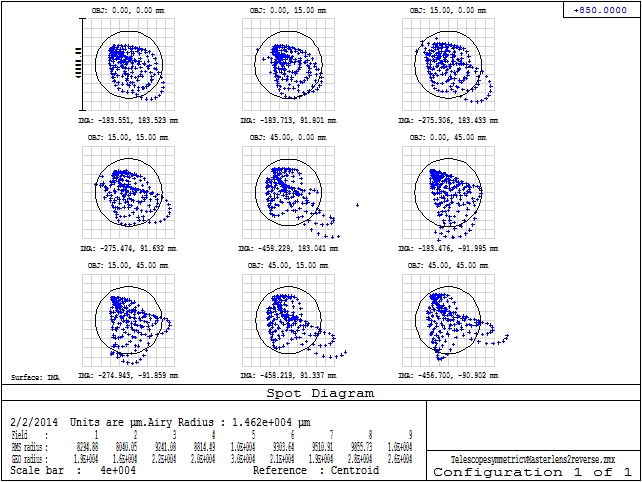
\includegraphics[width=3in]{images/ch4-zemax-spot-1-1.JPG}
\end{tabular}
\caption{
\ZEMAX\ spot diagrams for the \Imager's optical system.
The system was focused to \SI{16}{\m}.
This represents the distribution of points that rays trace to on the farfield focal plane.
Each plot shows spot diagrams for nine points in the focal planei covering the area over which detectors in the subarray are located.
The four plots (moving left to right and top to bottom) are for the secondary mirror with no tilt, \ang{1} tilt about one axis, \ang{1} title about other axis, and \ang{1} tilt about both axes.
The black circle gives \ZEMAX's estimate of the size of the Airy disk for the optical system, which is defined as the location of the first null is the system's diffraction pattern.
In all cases, nearly all rays map to within the Airy disk, indicating that the performance of the optical system is diffraction-limited.
}
\label{fig:ch4-spot-diagrams}
\end{figure*}


\section{Feedhorn Design}\label{sec:ch4-feedhorn-design}

% xxx where do I explain the choice of a square grid? Ans: section 6.3
% xxx where do I explain the missing 20 detectors?

Millimeter and submillimeter astronomical instruments using \TES\ detectors use many different strategies for coupling light onto detectors: filled arrays of absorbers \cite{swetz_overview_2011,holland_scuba-2:_2013}, antennas with lenslets \cite{keating_ultra_2011}, phased antenna arrays \cite{obrient_antenna-coupled_2012}, corrugated feedhorns \cite{austermann_sptpol:_2012,niemack_actpol:_2010}, and smooth-walled conical feedhorns \cite{schwan_invited_2011,sptxxx}.
The \Imager\ uses smooth-walled feedhorns because they are easy to design and easy to machine.
Smooth-walled feedhorns do not have the low cross-polarization properties of corrugated feedhorns \cite{clarricoats_corrugated_1984}, but this is not a concern here because the \Imager\ is polarization-insensitive.

\figref{fig:feedhorn-parms} depicts a smooth-walled conical feedhorn and its interaction with the optical system.
Although the optical system has a secondary mirror as well, for the purposes of feedhorn design the secondary mirror can be ignored and the system treated as a system of feedhorns illuminating only a primary mirror with a hole in its center \cite{xxxgoldsmith}.
If a feedhorn is observing a temperature distribution $T_{target}(\theta,\phi)$, and is pointed in a direction $(\theta_0, \phi_0)$, then the temperature observed by the feedhorn will be
\begin{equation}
    T_{eff}(\theta_0,\phi_0) = \int \, d \Omega \, T_{target}(\theta - \theta_0,\phi - \phi_0) P(\theta,\phi).
\end{equation}
The function $P$ is called the ``beam'' or ``beam pattern'' of the feedhorn, and describes the pattern of radiation to which the feedhorn is sensitive.
Although the \Imager\ is always receiving radiation, never transmitting, this thesis often writes about the beam pattern as if it were transmitting radiation, e.g.\ in decribing the portion of the ``beam'' that strikes the primary mirror.
This is acceptable because the transmitting and receiving beam patterns are exactly the same\footnote{This is a consequence of the reciprocity relationships obeyed by the Maxwell equations. See, e.g.\ \cite{balanis_antenna_2005} for a detailed explanation.}.
When using this expression one must keep in mind that the fraction of the beam that spills off the primary mirror (e.g.\ the unshaded region in \figref{fig:feedhorn-parms}) will see not the temperature distribution of the target, but a temperature distribution determined by what is beyond the primary mirror\footnote{Because of the presence of the secondary mirror, some of this temperature distribution will be in front of the system, and some will be behind.}.
The fraction of the beam that strikes the primary mirror and proceeds to the target is called the spillover efficiency $\eta_s$.

\begin{figure*}
\centering
\includegraphics{drawings/ch4-feedhorn-parms.pdf}
\caption{Schematic showing important parameters of a feedhorn and its beam. The beam appears to emerge from the phase center, a distance $l_c$ behind the mouth of the feedhorn in this diagram. The main lobe of the beam is approximated well by a Gaussian, here characterized by a full-width-half-maximum (\FWHM) beam width. The shaded fraction of the Gaussian represents the part of the beam that falls onto the primary mirror and reaches the target.}
\label{fig:feedhorn-parms}
\end{figure*}

The feedhorn opening diameter $D$ is chosen to minimize the total \NETD\ of the system.
The total \NETD\ was given in \sectionref{xxx} as
\begin{equation}
    NETD = \frac{NEP_{tot}}{2 k_B \Delta \nu \eta_{tot} \sqrt{2 \tau}}.
\end{equation}
To make the factors depending on the size of the feedhorns more clear we can break the optical efficiency $\eta_{tot}$ into a product of two factors, $\eta_s$ and $\eta_{other} = \eta_{tot} / \eta_s$.
We then note that the integration time per pixel $\tau$ is proportional to the number of detectors $N$.
This leads to
\begin{equation}
    NETD \propto \frac{NEP_{tot}}{\sqrt{N}\eta_s}.
\end{equation}

The critical relationship is that as a feedhorn's opening diameter increases, the width of the beam becomes smaller.
Small beam angles increase $\eta_s$, which improves \NETD.
However, the diffraction-limited area on the focal plane that can be covered by feedhorns is fixed, so that increases in the horn opening diameter reduce the number of detectors $N$, which worsens \NETD.
Choosing an optimal feedhorn size requires trading these two effect off against each other to minimize \NETD.

There are four additional factors to consider.
First, $NEP_{tot}$ is not neccesarily independent of $\eta_s$.
In a detector-noise limited system it will be, but in a system that is photon-noise-limted, $NEP_{tot}$ may worsen, stay the same, or improve, depending on the temperature seen by the spilled over portion of the beam.
Indoors all of the beam will see roughly the same temperature as the target, so that total photon noise will stay the same.
Outdoors the situation is more complicated because the temperature seen by the spilled over beam will depend on the local scenery and weather conditions.
For simplicity, the analysis of optimum feedhorn size in this chaper made the assumption that the noise seen by a detector is independent of the beam size.

Second, for a Cassegrain optical system, $\eta_s$ is not a monotonic function of $D$.
The secondary mirror obstructs the central part of the beam, preventing it from reaching the target.
This means that narrow beams can have poor $\eta_s$ because a large fraction of the main lobe of the beam will be blocked.

Third, the choie of readout system and wiring places a firm upper limit on the number of detectors in the system of 1024.

Fourth, the dependence of the number of detectors $N$ on the feedhorn diameter $D$ is not a smooth function, because it is not possible to have, e.g., 1/3 of a feedhorn.
As explained in \sectionref{xxx6.3}, the \Imager's detectors are laid out on a square grid.
So it is more helpful to think of the feedhorn diameter as taking on a discrete set of values that depends on the number of feedhorns per each side of the grid.

A \MATLAB\ program was used to find the optimum feedhorn size.
The program uses an analytic expression for the beam pattern developed in \cite{green_radiation_2006,narasimhan_modes_1971,}.
The far-field electric field pattern takes the form
\begin{equation}
    \vect{E}(\theta,\phi) = E_{\theta}(\theta) \sin{\phi} \hat{\theta} + E_{\phi}(\theta) \cos{\phi} \hat{\phi}.
\end{equation}
Here $E_{\theta}$ and $E_{\phi}$ are functions depending the horn diameter $D$ and opening half-angle $\alpha_0$, and involving definite integrals of Bessel functions, given in \appendixref{app:feedhorn-eqn}.
This expression is for the waveguide mode polarized along the $\pi/2$ direction.
The \Imager's detectors are unpolarized, so detect both waveguide polarizations equally (see \sectionref{xxx} for confirmation of this via simulations).
The total power beam map is thus given by the incoherant sum
\begin{equation}
    P(\theta, \phi) = (|\vect{E}(\theta, \phi)|^2 + |\vect{E}(\theta, \phi+\pi/2)|^2,
\end{equation}
which simplifies to 
\begin{equation}
    P(\theta) = |E_{\theta}(\theta)|^2 + |E_{\phi}(\theta)|^2,
\end{equation}
which is independent of $\phi$, as expected for an unpolarized detector.

To calculate the spillover efficiency of an individual feedhorn, the \MATLAB\ program integrates $P$ over the angles $\theta$ that illuminate the primary mirror and reach the target: \SIrange{5.3}{13.6}{\degree}\footnote{see \sectionref{sec:optical-design}}.
\figref{fig:ch4-feed-spill} shows a contour plot of spillover efficiency for an individual conical feedhorn as a function of $D$ and $\alpha_0$.
The blue asterisk matches the parameters for the feedhorns chosen for the \Imager.
This plot shows that $\eta_s$ depends much more strongly on $D$ than on $\alpha_0$.
$\alpha_0 = \SI{9.4}{\degree}$ was chosen as a value that is easy to machine, keeps the thermal mass of the feedhorn array relatively low (small values of $\alpha_0$ lead to long feedhorns and higher thermal mass), and it not too far from the maximum achievable $\eta_s$ for any fixed feedhorn diameter $D$.

\begin{figure*}
\centering
\includegraphics{./drawings/ch4-feed-spill.pdf}
\caption{
  Plot showing feedhorn spillover efficiency $\eta_s$ as a function of horn diameter $D$ and horn flare half-angle $\alpha_0$.
  The blue dotted line is for $\alpha_0 = \ang{9.4}$, the value assumed during optimization.
  The black dot shows the feedhorn parameters used in the \Imager: $D = \SI{2.68}{\mm}$ (cold) and $\alpha_0 = \ang{9.4}$
}
\label{fig:ch4-feed-spill}
\end{figure*}

To find the number of horns per array size that minimizes \NETD\, the program assumes that the the feedhorns must cover a square \SI{43.9}{\mm} per side.
It allows for \SI{1}{\mil} spacing between the edges of the feedorns, and also accounts for a thermal conctaction factor of 4.15 parts per thousand \cite{xxx}.
Four horns from each subarray are assumed to be missing in order to accomodate other features on the detector wafer.
The resulting \NETD\ estimates --- normalized to the NETD for the actual feedhorns chosen --- is shown in \figref{fig:ch4-netd-vs-nfeeds}.
The optimal number of feedhorns per array side is 19, for a total (across all four subarrays) of 1428 feedhorns of diameter \SI{2.25}{\mm} cold.
Because of readout limitations, the actual number of detectors per side is 16, for 1004 feedhorns with diameter \SI{2.68}{\mm} (\SI{108}{\mils} at room temperature).
The loss in \NETD\ from this suboptimal choice is only \SI{2}{\percent}.

\begin{figure*}
\centering
\includegraphics{./drawings/ch4-netd-vs-nfeeds.pdf}
\caption{
  Plot showing how \NETD\ depends on number of feedhorns in array.
  As discussed in the text, due to the square array the important parameter determining the total number of feedhorns is the number per side of the grid.
  The \NETD\ is plotted relative to the \NETD\ for an array with 16 feedhorns per side, which is the value chosen for this system.
  \NETD\ is minimized with 19 feedhorns per side, giving a total of 1428 feedhorns of diameter \SI{2.25}{\mm} (cold), but the \Imager\ uses 1004 feedhorns of diameter \SI{2.68}{\mm} (cold) because of readout limitations.
  The cost in \NETD\ is only \SI{2}{\percent}.
}
\label{fig:ch4-netd-vs-nfeeds}
\end{figure*}

% xxx - need to re-run all data analysis after verifying the proper
% inner angle!!!!

\figref{fig:ch4-beams} contains plots of both the beam pattern for the concial feedhorn and the far-field beam pattern of the entire optical system (also called the ``point spread function'').
The feedhorn beam pattern follows the model described above.
The far-field beam pattern accounts for the fact that the beam is truncated by the secondary mirror in it's center and by the edge of the primary at its edge; these limits are plotted as vertical blue lines on the left plot.
The truncation of the center of the beam is responsible for the sidelobe at \abt{\SI{}{\percent}} visible in the far-field beam pattern.
The far-field beam has a \FWHM\ of \SI{1.38}{\cm}.
After convolution with a \SI{0.2}{\in} circle the \FWHM\ is \SI{1.39}{\cm}, and after convolving with a \SI{1.791}{\cm} circle (same size as a dime) the \FWHM\ is \SI{1.76}{\cm}.

\begin{figure*}
\centering
\includegraphics{./drawings/ch4-beams.pdf}
\caption{
  Plot showed expected beam pattern for design feedhorns.
  \textbf{Left} The unpolarized power pattern for a conical feedhorn with diameter \SI{2.68}{\mm} and opening half-angle $\alpha_0 = \ang{9.4}$, at the center frequency for our band.
  The region between the vertical blue lines indicates the part of the beam that strikes the primary mirror and reaches the far-field focal plane.
  Also plotted is the best-fit Gaussian within the blue lines.
  The \FWHM beam width is \ang{10.6}.
  \textbf{Right} Far-field unpolarized power pattern.
  This accounts for blockage by the secondary mirror and well as the edge tape of the beam pattern on the primary.
  The sidelobe is caused by the secondary mirror, and is \SI{5.7}{\percent} high.
}
\label{fig:ch4-beams}
\end{figure*}

\section{Optical Coupling to Detectors}

\section{Predicted Optical Efficiency and Optical Loading on Detectors} \label{sec:ch4-opt-eff}
\begin{equation} \label{eqn:ch4-power-per-mode}
  \frac{2 h \nu}{e^{\frac{h \nu}{k_B T}} -1} \Delta \nu
\end{equation}
\section{Detector Readout} \label{sec:det-readout}

\section{Acknowledgments}

Bob Schwall and William Duncan of NIST designed the cryostat/mirror mount and the \He4 sorption refrigerator.
The refrigerator was filled with \He4 by Simon Dicker at the University of Pennsylvania.
Bob Schwall of NIST designed the cryostat, and provided useful advice and help in the lab during commissioning of the cryostat.
William Duncan designed, procured, and assembled the optical system.
Mandana Amiri and Matthew Hasselfield provided extensive, timely and invaluable support for the MCE hardware and software.

